\chapter{Implementation}

The implementation of our software is built on Chládek's source code from his diploma thesis \cite{chladek_thesis}. We apply his implementation of basic classes for defining the phylogenetic tree, parsing an unrooted gene tree and a rooted species tree from a file with several changes. We also use his implementation of the two-pass algorithm, which we mentioned before in Chapter \ref{two-pass_algorithm}, to compute the gene tree possible mapping depths.

On this basis, we implement our algorithms described in Chapter \ref{Algorithms} to find the most parsimonious reconciliation.

Our software is implemented in the programming language Java and has a command-line interface.

\section{Classes and variables}
%variables
The implemented software consists of 15 classes that we briefly introduce:
\begin{itemize}
  \item Class Node - represents a node in a phylogenetic tree
  \item Class Edge - represents an edge in a phylogenetic tree
  \item Class Interval - represents a length of edge as interval
  \item Class DL - represents a score of reconciliation
  \item Class UnrootedNode - represents a node in an unrooted gene tree
  \item Class UnrootedTree - represents an unrooted gene tree
  \item Class RootedExactNode - represents a node in a rooted species tree with exact branch lengths
  \item Class RootedExactTree - represents a rooted species tree with exact branch lengths
  \item Class RootedIntervalNode - represents a node in a rooted gene tree with inexact branch lengths
  \item Class RootedIntervalTree - represents a rooted gene tree with inexact branch lengths
  \item Class Parser - parses phylogenetic trees and their leaf-mapping from files
  \item Class Loader - load arguments from a command line and calls Parser on files with stored phylogenetic trees
  \item Class Printer - prints reconciliation solutions into files
  \item Class Reconciliator - computes reconciliation with its score
  \item Class Main - the main class of the software that calls other classes to load files, compute and print reconciliation
\end{itemize}

\section{Differences from the original source code}

As our source code is built on Chládek's source code, we show the differences in relations and entities between source codes in Fig. \ref{relation_diagram}. The differences, new variables and classes are described below by classes in more details.\\
\begin{figure}[ht!]
	\centering
	\label{relation_diagram}
  	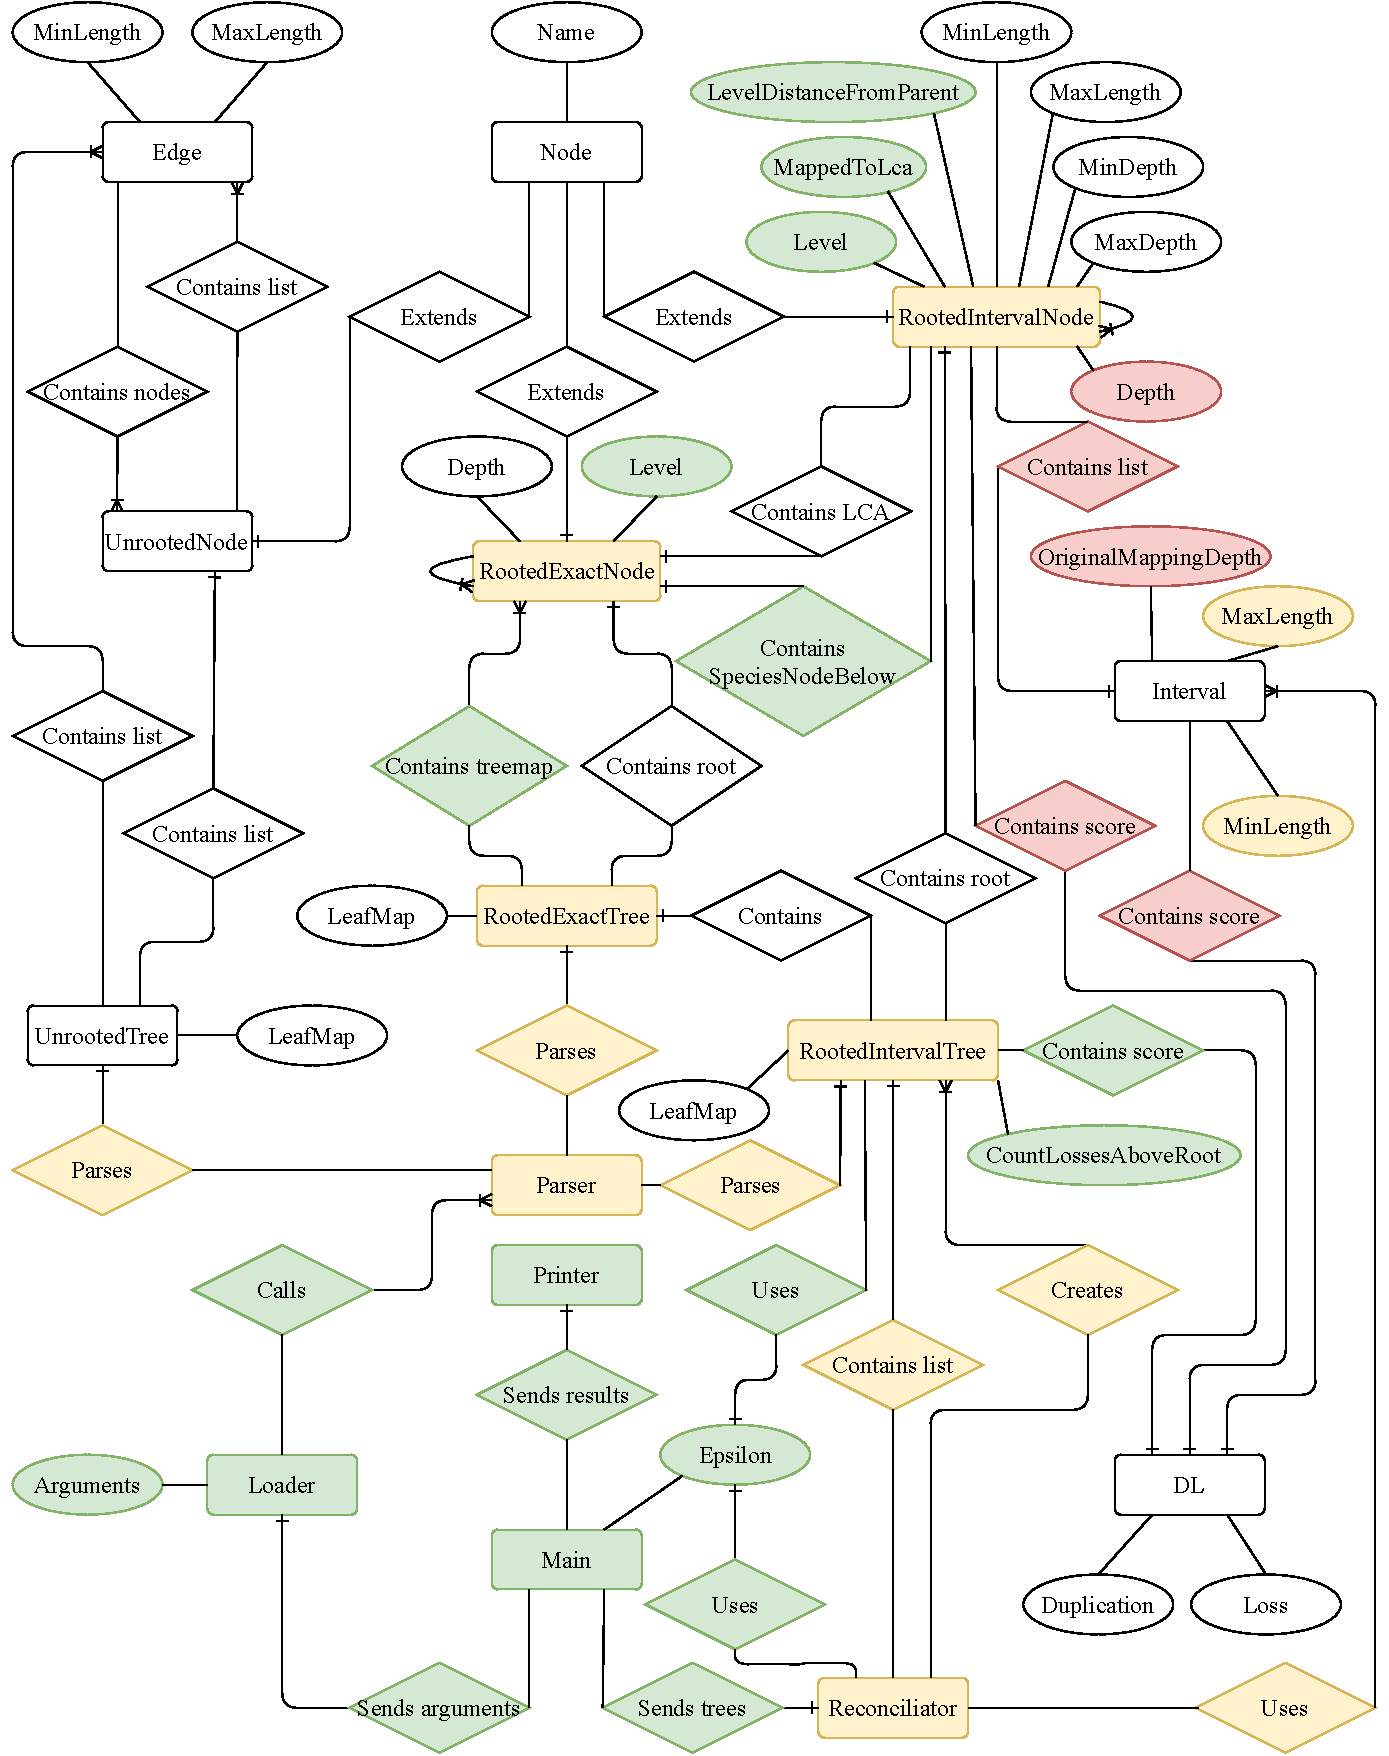
\includegraphics[width=\linewidth]{relation_diagram}
  	\caption[Entity-relationship diagram with differences]{Red entities and relations represent deleted variables or functions. Yellow entities and relations show changes to the original source code. Green entities and relations depict added classes, variables or functions.}
\end{figure}
\textbf{Class Interval}

We change the name of parameters to \emph{minLength} and \emph{maxLength} and delete the unnecessary variable \emph{OriginalMappingDepth} as we use the \emph{Interval} to store the minimal and maximal length of new possible edges that can be created after subdividing the original root edge in function\emph{getIntervals} (Algorithm \ref{getIntervals}) in \emph{Reconciliator} class. The parameters are numbers of type double.\\
\textbf{Class RootedExactNode}

In the \emph{RootedExactNode} class, we define a new \emph{level} variable. It is a number of type integer. The variable is set while parsing the species tree in the \emph{Parser} class and used for computing the level of gene nodes as shown in function \emph{computeLevel} (Algorithm \ref{computeLevel}) in \emph{Reconciliator} class.\\
\textbf{Class RootedExactTree}

We add structure \emph{TreeMap} containing leaves, where the key is the name of the leaf and the value is an object representation of that leaf as \emph{RootedExactNode}. It is used to set the LCA-mapping variable of leaves in a gene tree according to the leaf-mapping.\\
\textbf{Class RootedIntervalNode}

The unnecessary \emph{depth} variable was deleted as we store the mapping depth of a \emph{RootedIntervalNode} in variables \emph{minDepth} and \emph{maxDepth}. We also delete the \emph{DL}, because we do not store the reconciliation score in nodes and the list of \emph{Interval} since we have the mapping depth interval and the interval of the edge above stored in separated variables. Besides, we add new variables: \emph{level}, \emph{mappedToLca}, \emph{levelDistanceFromParent} and \emph{speciesNodeBelow} that are computed and used in algorithms in Chapter \ref{counting_algorithm}. The \emph{level} and \emph{levelDistanceFromParent} are numbers of type integer. The \emph{mappedToLca} is data type boolean \emph{speciesNodeBelow} is object of type \emph{RootedExactNode}.\\
\textbf{Class RootedIntervalTree}

In the \emph{RootedIntervalTree}, we implement our algorithms from Chapter \ref{counting_algorithm} and their are called from the \emph{Reconciliator} class. We add the variable of type \emph{DL} to store the number of duplication and gene losses inferred in the gene tree.\\
\textbf{Class Parser}

We change the parsing method for a species tree and an unrooted gene tree. In the species tree parsing method, we infer \emph{level} in species tree nodes. In the unrooted gene tree parsing method, we resolve inexact branch lengths if the given gene tree has inexact branches or we transform exact branch lengths to inexact branch lengths if the given gene tree has exact branch lengths. To modify the exact branch lengths into inexact branch lengths, the user needs to set the tolerance value that has to be from interval $[ 0, 1 ]$. The interval of the edge is compute as: $[ length - (tolerance \cdot length), length + (tolerance \cdot length) ]$.

Furthermore, we add a parsing method for a rooted gene tree that can either resolve inexact branch lengths or transform exact branch lengths to inexact branch lengths. We included a method to parse mapping of gene leaves to species leaves from a file and a method for transforming a rooted gene tree to an unrooted gene tree. This allows us to forget the original root of a gene tree and find a new one with function \emph{getIntervals} (Algorithm \ref{getIntervals}). All methods in the class are called from the \emph{Loader} class.\\
\textbf{Class Loader}

The \emph{Loader} class is initialized with arguments from the command line. It loads the arguments and calls functions from \emph{Parser} according to the requirements specified in the arguments. We recognize 11 arguments that are listed in Table \ref{arguments}.

\begin{table}[ht!]
\caption{Input arguments}
\centering
  \begin{tabular}{| m{0.25\textwidth} | m{0.65\textwidth} |}
  \hline
    \textbf{Argument}  & \textbf{Description}\\
    \hline
    -help & shows help information with all possible input arguments \\
    \hline
    -S <species tree> & path to the rooted species tree file in Newick tree format (mandatory input)\\
    \hline
    -G <gene tree> & path to the rooted or unrooted gene tree in Newick tree format (mandatory input)\\
    \hline
    -M <species map> & mapping of genes to species\\
    \hline
    -t <tolerance> & required tolerance from interval $[ 0, 1 ]$ (By default, it is set to $0.5$) \\
    \hline
    -s <step> & required step from $[0, \infty]$ (By default, it is set to $0.01$)\\
    \hline
    -r & signifies that the given gene tree is rooted (By default, the given gene tree is considered to be unrooted)\\
    \hline
    -reroot & signifies that the given rooted gene tree is wished to be rerooted\\
    \hline
    -l & signifies counting the gene losses above the root of given gene tree\\
    \hline
    -p <print type> & required print type from two options \emph{"sol"} and \emph{"rel"} (By default, the print type is set to be \emph{"sol"}\\
    \hline
    -epsilon <epsilon> & required epsilon as number of type double (By default, it is set to \num{1e-6}\\
    \hline
  \end{tabular}
  \label{arguments}
\end{table}

The main method is \emph{loadArgs} which is called from the \emph{Main} class and returns an array of \emph{Object}: a rooted species tree, a rooted gene tree or an unrooted gene tree, \emph{step} and \emph{countLossesAboveRoot} needed for algorithms from Chapter \ref{counting_algorithm} implemented in \emph{Reconciliator} class along with \emph{dirPathGene} and \emph{printType} required in \emph{Printer} class functions.\\
\textbf{Class Reconciliator}

The algorithms from Chapter \ref{Algorithms} and the two-pass algorithm by Chládek from Chapter \ref{two-pass_algorithm} are called in the \emph{Reconciliator} class. These are the main methods to obtain the most parsimonious reconciliation.

The \emph{Reconciliator} class is initialized with a rooted species tree, a rooted gene tree or an unrooted gene tree, \emph{step} and \emph{countLossesAboveRoot} that are inferred in \emph{Loader} class. It uses \emph{Interval} to store the minimal and maximal length of new edges in function \emph{getIntervals} (Algorithm \ref{getIntervals}), which are used for subdividing the root edge and creating the \emph{RootedIntervalTree}. The class returns a list of \emph{RootedIntervalTree} with most parsimonious reconciliation that has its reconciliation score store in \emph{DL}.\\
\textbf{Class Printer}

The class is initialized with list of \emph{RootedIntervalTree}, \emph{dirPathGene} and \emph{printType}. We recognise two types of printing the results of the reconciliation into the file: \emph{"rel"} and \emph{"sol"}.

With the \emph{"rel"} type, the function prints relations between genes in the gene tree for each inferred \emph{RootedIntervalTree}. If solutions contain more trees with the same topology and reconciliation score, it prints the number of the same tree after each gene relation printout. For each $u \in L(G)$, it prints \emph{"gene"} and name of the node $u$. For each $v \in V(G)\setminus L(G)$, it allows evolutionary events as speciation, duplication and gene loss depending on what occurred in the node $v$ or on the branch from the node $v$ to its parent $parent(v)$. The speciation and duplication are inferred in the node $v$. They print as \emph{"spec"} for speciation and \emph{"dup"} for duplication with names of $children(v)$ separated by a tab. The gene loss happens on the branches. It prints as \emph{"loss"} with the name of node $v$. The name of each node consists of genes found in the subtree of that node separated by commas. 

The \emph{"sol"} type prints gene trees in special Newick format, where branch lengths are inexact. All computed solutions are printed into one \emph{.txt} file, where solutions are separated with an empty line.

The file with results is saved in the same directory as the given gene tree.\\
\textbf{Class Main}

The \emph{Main} class receives arguments given by user and send it to the \emph{Loader} class for processing. Sequentially, sends a rooted species tree, a rooted gene tree or an unrooted gene tree, \emph{step} and \emph{countLossesAboveRoot} to the \emph{Reconciliator} class to infer the most parsimonious reconciliation, which returns list of \emph{RootedIntervalTree}. Eventually, it sends the list of \emph{RootedIntervalTree}, \emph{printType} and \emph{dirPathGene} to the \emph{Printer} to print the results. Also, it stores the value of $\epsilon$ that are required in functions \emph{getIntervals} (Algorithm \ref{getIntervals}) in \emph{Reconciliator} class and \emph{computeLevel} (Algorithm \ref{computeLevel}) in \emph{RootedIntervalTree} class.  \\
